\documentclass[11pt,a4paper]{article}
\usepackage{a4wide,graphicx,enumitem}
\usepackage[utf8]{inputenc}
\usepackage{hyperref}

\parindent0pt
\parskip4pt

\title{The Toyota Management System. \\ Guiding Principles and Main Tools}

\author{Toni Pfeiffer\\
  Universität Leipzig\\
  Seminar Complex Systems and Co-operative Action
}

\date{June 22, 2021}

\begin{document}
\maketitle

\section{Introduction}
This handout refers to the book "The Toyota Way -- 14 Management Principles of
the World's Most Successful Automotive Company" by Jeffrey K. Liker
\cite{toyota_book}.  Jeffrey Liker has followed the company for 20 years and
summarized his knowledge about it in the book. He analyzed Toyota's success
and discovered 14 methods that enabled Toyota to become the most successful
automotive company in the world. In order to understand the success of Toyota,
it is necessary to look at the history of the company.This will be described
in more detail in the next chapter. The Toyota Production System, another
component of success, will be described only briefly.  Here we will focus on
the management methods that describe Toyota's holistic approach. The
individual principles were divided by Liker into 4 categories, also called the
4 P's. Philosophy, Processes, People/Partners and Problem Solving. These
categories can be thought of as a pyramid to be seen in \autoref{fig:4P}.
Problem solving is the top of the pyramid. The most important is the
foundation, the philosophy of the company. This philosophy runs through all
management levels and eras. Starting with the founding Toyoda family, which is
described in more detail below.

\section{History of Toyota}

Toyota's history began with Sakichi Toyoda. He started to build looms in
1894. Soon he bought a used steam engine and experimented with it to build a
power loom. Together with his son Kiichiro Toyoda, he succeeded. He sold the
patent for his automatic loom in Great Britain and got the start-up capital to
found Toyoda Automatic Loom Inc. In 1936, the first car model was launched.
The company was then renamed Toyota Motor Corporation. Fortunately, the
company was able to survive the 2nd World War unscathed. Nevertheless,
difficulties arose due to inflation. Kiichiro had to lay off staff. He also
left the company and made room for his cousin Eiji Toyoda. Eiji Toyoda made
several trips to automobile manufacturers in the USA and returned with the
task of outperforming them. He shared this task with Taiichi Ohno, the plant
manager, who then developed the Toyota Production System. This system is
illustrated in \autoref{fig:TPS}. The cornerstones of success are based on
this system. Stable and standardized processes, visual management, and
Toyota's philosophy form the foundation. The pillars are the Just-In-Time
principle, Jidoka, people and the elimination of non-value elements. This
system leads to the best quality, lowest cost, highest safety and high
morale. All steps and processes must be seen as a whole. For example,
just-in-time deliveries may lead to performance improvements, but may not be
beneficial in the long run. It is necessary to constantly analyze and improve
the processes. This is what the upcoming managers of Toyota did. They improved
processes and introduced principles that increased Toyota's success. All
driven by the philosophy and the 14 principles explained below.

\begin{figure}[h] 
  \centering
     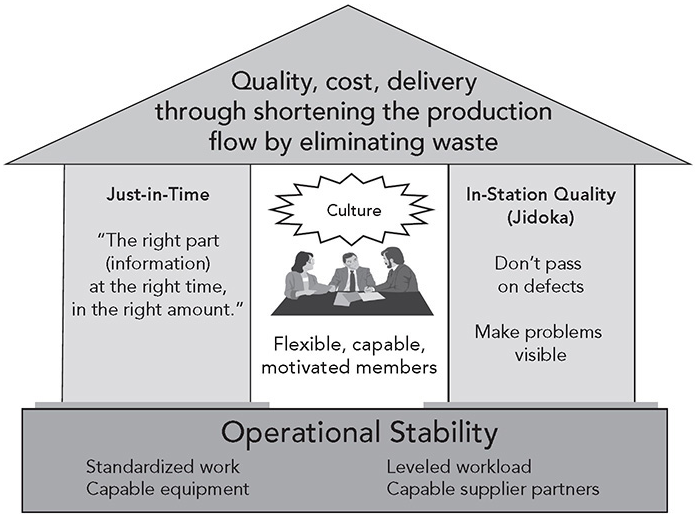
\includegraphics[width=0.7\textwidth]{toyota_production_system.png}
  \caption{The Toyota Production System}
  \label{fig:TPS}
\end{figure}

\section{Principles}

Jeffrey K. Liker divides the principles into four categories -- Philosophy,
Processes, People and Partners, and Problem Solving. These four categories
contain the principles that made Toyota successful. In \autoref{fig:4P} you
can see the pyramid that Liker describes. The foundation is the philosophy
which is now described first.

\begin{figure}[h] 
  \centering
     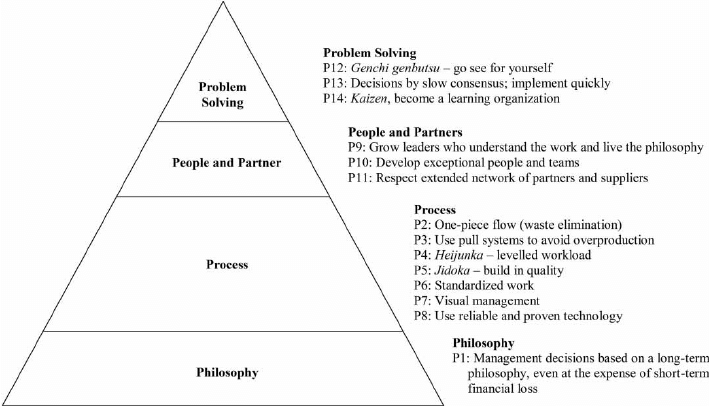
\includegraphics[width=0.7\textwidth]{4P.png}
  \caption{The Toyota Way Model}
  \label{fig:4P}
\end{figure}

\subsection{Philosophy}

\begin{enumerate}
\item[1.] \textbf{Principle: Long-term thinking}
  
  Base your management decisions on a long-term philosophy, even if it is at
  the expense of short-term profit targets. Toyota's major goals are to
  generate value for the customer, society and the economy.

  Toyota's philosophy is summarized by Liker in 7 points.
  \begin{itemize}
  \item Honor the language and spirit of the law of every nation and undertake
    open and fair corporate activities to be a good corporate citizen of the
    world.
  \item Respect the culture and customs of every nation and contribute to
    economic and social development through corporate activities in the
    communities.
  \item Dedicate ourselves to providing clean and safe products and to
    enhancing the qualitiy of life everywhere through all our activities.
  \item Create and develop advanced technologies and provide outstanding
    products and services that fulfill the need of customers worldwide.
  \item Foster a corporate culture that enhances indiviual creativity and
    teamwork value, while honoring mutual trust and respect between labor and
    management.
  \item Pursue growth in harmony with the global community through innovative
    management.
  \item Work with business partners in research and creation to achieve
    stable, long-term growth and mutual benefits, while keeping ourselves open
    to new partnerships.
  \end{itemize}  
\end{enumerate}

\subsection{Process}

\begin{enumerate}
\item[2.] \textbf{Principle: One-Piece Flow}

  The main goal here is the elimination of superfluous things, also called
  muda. These muda, according to Liker, can be the following things:
  \begin{itemize}[noitemsep]
  \item Overproduction
  \item Waiting
  \item Unnecessary transport
  \item Overprocessing
  \item Excess inventory
  \item Unnecessary movement
  \item Defects
  \item Unused employee creativity
  \end{itemize}
  \begin{figure}[h] 
    \centering
    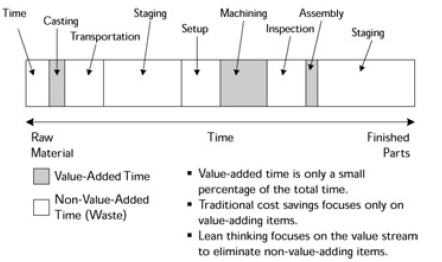
\includegraphics[width=0.7\textwidth]{waste.PNG}
    \caption{Waste in a value system}
    \label{fig:waste}
  \end{figure}
    
  In \autoref{fig:waste} you can see the wastes in a value system. If you
  eliminate them, you can get the following advantages:
  \begin{itemize}[noitemsep]
  \item Build-in quality
  \item Creates real flexibility
  \item Creates higher productivity
  \item Frees up floor space
  \item Improves safety
  \item Improves moral
  \item Reduces cost of inventory
  \end{itemize}
    
\item[3.] \textbf{Principle: Pull-System}
  
  The main goal of the pull system is to make what's needed when it is needed.
  So you can get advantage of small storage costs.
    
\item[4.] \textbf{Principle: Heijunka: Balanced Workload}

  Heijunka tools attempt to balance workload and production volume.  Yamazumi
  balances workload within a production process. A balance in both areas leads
  to a continuous flow of work and materials, from transport to the customer
  at the end of the chain, to material deliveries from suppliers at the
  beginning of the chain.

\item[5.] \textbf{Principle: Jidoka: Build-in quality}

  Create a culture that produces quality right away, rather than a culture of
  perpetual rework. Providing customers with quality drives your value
  proposition. Use all available modern quality assurance methods. Equip your
  machines to be able to identify problems and shut down automatically.
  Develop a visual system that notifies a team or project manager when a
  machine or process needs help. Jidoka (self-directed error detection) is the
  foundation of "in-process" quality.  Establish support systems in your
  organization for rapid problem resolution, and take resolution action.
  Incorporate into your culture a philosophy of deceleration or interruption
  of production to get quality right the first time, thus increasing
  productivity in the long run.

\item[6.] \textbf{Principle: Standardized work}

  Standardized work steps are the foundation for continuous improvement and
  the transfer of responsibility to employees. Use stable, repeatable methods
  everywhere to ensure predictability, regular timing, and regular results
  from your processes. This is the basis for fluid processes and pull effects.
  Capture cumulative learning about a process by making best practices the
  standard. Give room for creative, individual expression to further improve
  the standard, and incorporate that improvement into the new standard. This
  way, you can transfer the learning to a successor when an employee leaves
  the company.
    
\item[7.] \textbf{Principle: Visual Management}

  Use visual controls to ensure that no problems remain hidden.  Use simple
  visual signaling devices to help your workers decide if it's a standard
  situation or an anomaly. Eliminate computer screens if they distract your
  workers' attention from their workstations.  Develop simple visual systems
  at individual workstations to support fluid processes and pull effects.
  Wherever possible, reduce your reports to one page, even for your most
  important financial decisions.

\item[8.] \textbf{Principle: Use only reliable technology}

  Use only reliable, thoroughly tested technologies that serve people and
  processes. Use technology to support people, not replace them. It is often
  best to execute a process manually before adding technological support. New
  technologies are often unreliable and difficult to standardize. Therefore,
  they put the "flow" at risk. A proven process that works reliably is far
  preferable to a new untested technology. Conduct testing before introducing
  new technologies into business processes, manufacturing systems, or
  products. Eliminate or modify technologies that conflict with your culture
  or that threaten the stability, reliability or predictability of the system.
  Nonetheless, encourage your employees to engage with new technologies as
  they seek new approaches. Deploy a thoroughly tested technology quickly if
  it has been proven in testing to improve your process flow.
\end{enumerate}

\subsection{People}

\begin{enumerate}
\item[9.] \textbf{Principle: Leaders}
  
  Grow leaders who thoroughly understand the work, live the philosophy and
  teach it to others. Develop leaders from within your own ranks instead of
  buying in external leaders. Don't think of the leadership role as simply
  performing certain tasks and being able to deal well with people. Leaders
  must serve as role models for a lived corporate philosophy and for the way
  the company does business. A good business leader must be intimately
  familiar with the details of day-to-day business. Only then he can be the
  best teacher of the corporate philosophy.

\item[10.] \textbf{Principle: People and Teams}
  
  Develop exceptional people and teams who follow your company‘s philosophy.
  Create a strong and stable culture where corporate values and beliefs are
  shared by all and actively lived for many years. Train above-average
  employees and teams to work in line with the corporate philosophy to achieve
  exceptional results. Work hard to continually strengthen the culture. Use
  interdisciplinary teams to improve quality and productivity and increase
  process flow by solving difficult technical problems. Ownership happens when
  employees use the tools of the business to improve the business. Work
  tirelessly to show individual employees how to work as a team toward a
  common goal. Teamwork is something that must be learned.

\item[11.] \textbf{Principle: Network}
  
  Respect your extended network. Respect your business partners and suppliers,
  and treat them like an extension of your company.  Challenge your external
  business partners to grow and develop. This shows your appreciation. Set
  challenging goals and support your partners in achieving them.
\end{enumerate}

\subsection{Problem solving}

\begin{enumerate}
\item[12.] \textbf{Principle: Genchi Genbutsu}
  
  Solve problems and improve processes by getting to the root of the problem
  and personally verifying information, rather than writing theoretical papers
  based on second-hand information or computer data. Everything you say and
  think should be based on data you have personally verified. Even
  high-ranking managers and executives should personally see things for
  themselves so that they fully understand the situation.

\item[13.] \textbf{Principle: Nemawashi -- make decision}
  
  Make decisions wisely and according to the consensus principle. Weigh all
  alternatives carefully, but implement the decision made expeditiously. Do
  not become rigid about a direction and take that course before you have
  thoroughly considered the alternatives. Once you have decided on an
  alternative, follow that course briskly but carefully. Nemawashi is the
  process of discussing the problems and their potential solutions with all
  stakeholders to gather their ideas and gain agreement on a solution. This
  consensus-based process is time-consuming, but opens up more avenues for
  solutions. And once the decision is made, the conditions are in place for
  rapid implementation.

\item[14.] \textbf{Principle: Kaizen -- continuous improvements}
  
  Become a truly learning organization through relentless reflection (hansei)
  and continuous improvement (kaizen). Once you have a robust process in
  place, use continuous improvement tools to identify the root causes of
  inefficiencies and implement effective countermeasures. Develop processes
  that require virtually no inventory. This will make wasted time and wasted
  resources visible to all. When waste becomes visible, get your staff to
  continuously improve processes (kaizen) to eliminate the waste. Protect
  institutional knowledge by ensuring a stable workforce, slow promotion, and
  very careful succession systems. Use hansei (reflection) when you reach
  certain milestones and after a project is completed to reveal any
  shortcomings of the project. Develop countermeasures to avoid repeating the
  same mistakes. Learn by making best practices the standard, rather than
  reinventing the wheel with each new project and each new manager.
\end{enumerate}
\begin{thebibliography}{99}
\bibitem{toyota_book} Jeffrey K. Liker \emph{Der Toyota Weg; 14
  Managementprinzipien des weltweit erfolgreichsten Automobilkonzerns},
  8. Auf\-lage. Finanzbuchverlag, München, 2013.
\end{thebibliography}
\end{document}
